\documentclass{article}
\usepackage[utf8]{inputenc}
\usepackage[francais]{babel}
\usepackage[T1]{fontenc}
\usepackage{graphicx}    
\usepackage{eurosym}
\usepackage{verbatim}      
\usepackage{amsmath, amsthm}                             
\usepackage{latexsym}                               
\usepackage{amssymb}
\usepackage{tabularx}
\usepackage{setspace}
\usepackage{listings}
\usepackage{geometry}
\usepackage{fancyhdr}
\usepackage{enumitem}
\usepackage{colortbl}
\usepackage[dvipsnames]{xcolor}
\usepackage{booktabs} 
\usepackage{moreverb}

\DeclareMathAlphabet{\mathonebb}{U}{bbold}{m}{n}
\newcommand{\one}{\ensuremath{\mathonebb{1}}}

\usepackage{color}
\usepackage{multirow}
%\usepackage{float}
\definecolor{gris25}{gray}{0.75}
\usepackage{colortbl}
\usepackage{fancyhdr}
\usepackage{amsmath,amsfonts,amssymb}
\usepackage{titlesec}
\usepackage{supertabular}
\usepackage{longtable}

\usepackage{caption}
\usepackage{subcaption}


\usepackage{listings}
\definecolor{dkgreen}{rgb}{0,0.4,0}
\definecolor{gray}{rgb}{0.5,0.5,0.5}
\definecolor{mauve}{rgb}{0.58,0,0.82}

\usepackage{algorithm2e}

\usepackage{hyperref}
\hypersetup{
    colorlinks=true,
    linkcolor=blue,
    filecolor=magenta,      
    urlcolor=blue,
}
 
\urlstyle{same}

\definecolor{dkyellow}{cmyk}{0, 0, 0.2, 0}
\lstset{
  language=Python,                % the language of the code
  basicstyle= \footnotesize,      % the size of the fonts that are used for the code
  numbers=left,                   % where to put the line-numbers
  numberstyle=\tiny\color{gray},  % the style that is used for the line-numbers
  stepnumber=2,                   % the step between two line-numbers. If it's 1, each line 
                                  % will be numbered
  showspaces=false,               % show spaces adding particular underscores
  showtabs=false,                 % show tabs within strings adding particular underscores
  frame=single,                   % adds a frame around the code
  rulecolor=\color{black},        % if not set, the frame-color may be changed on line-breaks within not-black text (e.g. commens (green here))
  tabsize=2,                      % sets default tabsize to 2 spaces
  captionpos=b,                   % sets the caption-position to bottom
  breaklines=true,                % sets automatic line breaking
  breakatwhitespace=false,        % sets if automatic breaks should only happen at whitespace
  keywordstyle=\color{blue},      % keyword style
  commentstyle=\color{dkgreen},   % comment style
  stringstyle=\color{mauve},       % string literal style
  backgroundcolor=\color{white},      % choose the background color. You must add \usepackage{color}
}

\usepackage{array}
\newcolumntype{L}[1]{>{\raggedright\let\newline\\\arraybackslash\hspace{0pt}}m{#1}}
\newcolumntype{C}[1]{>{\centering\let\newline\\\arraybackslash\hspace{0pt}}m{#1}}
\newcolumntype{R}[1]{>{\raggedleft\let\newline\\\arraybackslash\hspace{0pt}}m{#1}}

\usepackage{xcoffins}
\NewCoffin\tablecoffin
\NewDocumentCommand\Vcentre{m}
  {%
    \SetHorizontalCoffin\tablecoffin{#1}%
    \TypesetCoffin\tablecoffin[l,vc]%
  }



\begin{document}
%%%%%%%%%%%%%%%%%%%%%%%%%%%%%%%%%%%%%%%%%%%%%%%%%%%%%%%%%%%%%%%
\begin{titlepage}

%  \begin{center} 
%    \textsc{ENSAE ParisTech}\\
%    ---\\
%    Année 2013--2014
%  \end{center}
  
\begin{center}

\includegraphics[width=0.3\textwidth]{Mines_ParisTech.png} 

\includegraphics[width=0.3\textwidth]{CURIE.jpg}

\includegraphics[width=0.3\textwidth]{INSERM.jpg}
\end{center}

\vspace{\stretch{1}}
 
\noindent
\hrulefill
  \begin{center} \bfseries\Huge
Towards image-based cancer signatures from histopathology data
  \end{center}
  \begin{center} \huge
   First year report
  \end{center}
\hrulefill 
  
  \vspace{\stretch{2}}
   \begin{center}  \large
\textit{Supervisor} : \textsc{T. Walter and F. Reyal}. \\
\textit{Units:} \textsc{Center for Computational Biology and UMR900}

   \end{center}
     
  \vspace{\stretch{3}}
  \begin{center} \Large
  Peter \textsc{Naylor}
  \end{center}

  \vspace{\stretch{4}}

  \begin{center}  \large
    June 2016
  \end{center}

\end{titlepage}
%%%%%%%%%%%%%%%%%%%%%%%%%%%%%%%%%%%%%%%%%%%%%%%%%%%%%%%%%%%%




\newpage
\tableofcontents
\newpage

\section{Introduction}

\subsection{Context}

\subsection{PhD subject}

\section{November 2015 - January 2016: MitoCheck Project}

\section{January 2016 - April 2016: Camelyon2016 challenge}

This Challenge is organized in conjunction with and with the support of the 2016 IEEE International Symposium on Biomedical Imaging  (ISBI-2016) and this the first challenge using whole-slide images in histopathology. This challenge fitted particularly well with my PhD time table as the data used in this challenge is very similar to the data acquired by F. Reyal. Our final ranking was not very satisfying as we did not achieve good results. This work was done with the help of V. Machairas, T. Walter and E. Decenciere. A website was made for the purpose of this challenge, \url{http://camelyon16.grand-challenge.org/home/}.

\subsection{Context}
The goal of this challenge is to evaluate new and existing algorithms for automated detection of metatases in hematoxylin and eosin (HE) stained whole-slide images of lymph node sections, see figure \ref{LymphNode} This task has a high clinical relevance but requires large amounts of reading time from pathologists. Therefore, a successful solution would hold great promise to reduce the workload of the pathologists while at the same time reduce the subjectivity in diagnosis. The Camelyon2016 challenge will focus on sentinel lymph nodes of breast cancer patients and 2 large datasets have been provided from both the Radboud University Medical Center (Nijmegen, the Netherlands), as well as the University Medical Center Utrecht (Utrecht, the Netherlands). The focus on lymph nodes of breast cancer patients is not arbitrary, lymph node metastases occur in most cancer types (e.g. breast, prostate, colon). Lymph nodes are small glands that filter lymph, the fluid that circulates through the lymphatic system. The lymph nodes in the underarm are the first place breast cancer is likely to spread. Metastatic involvement of lymph nodes is one of the most important prognostic variables in breast cancer. Prognosis is poorer when cancer has spread to the lymph nodes.


\begin{figure}[!ht]
\centering
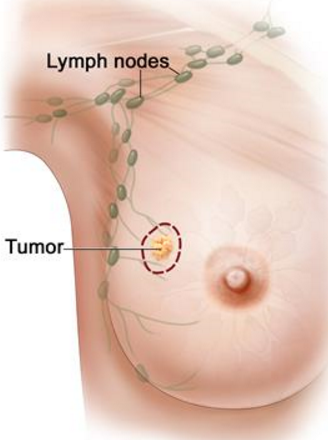
\includegraphics[width=0.4\textwidth]{Booby.png}
\caption{Lymph nodes}
\label{LymphNode}
\end{figure}

\begin{figure}[!ht]
\centering
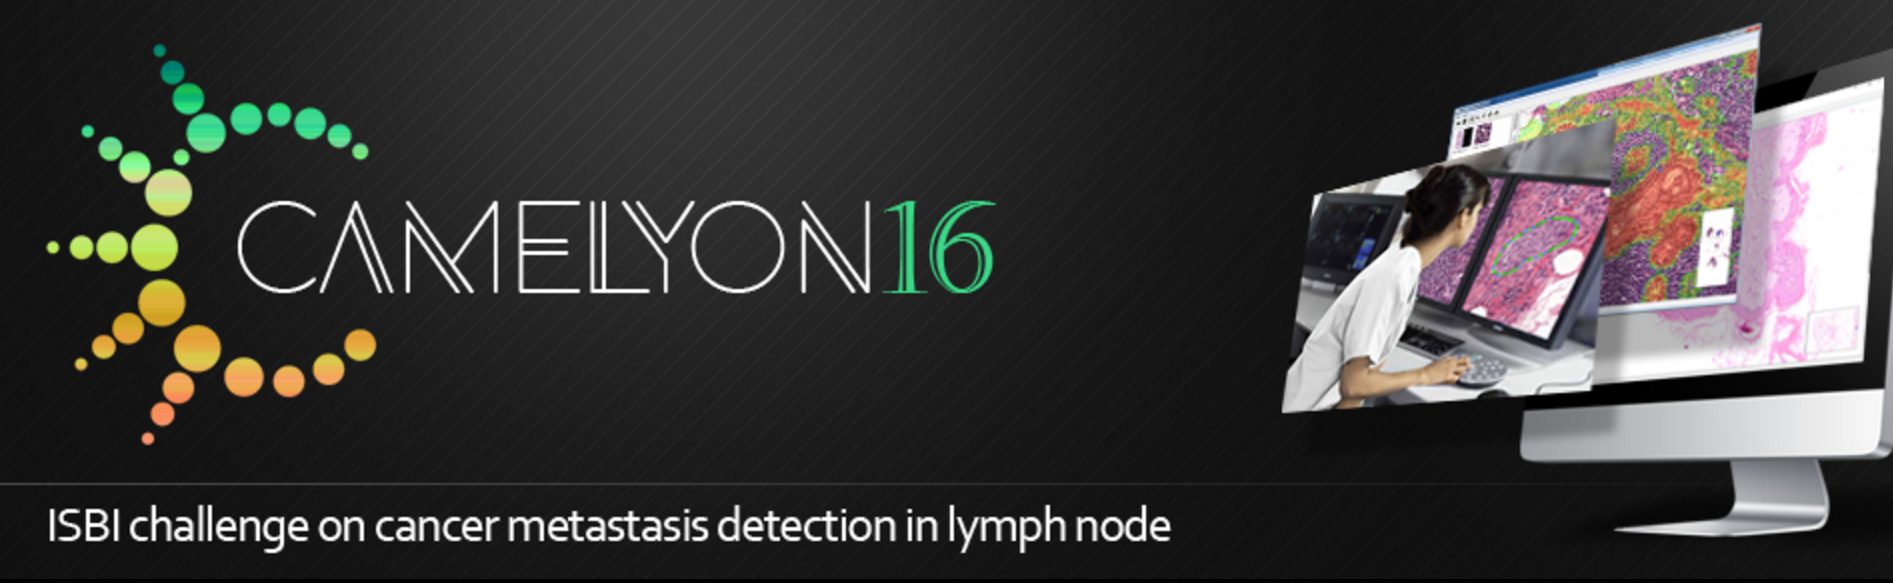
\includegraphics[width=\textwidth]{Camelyon16.png}
\caption{Official logo}
\label{Ol}
\end{figure}
\subsection{Work pipeline}
Some of the decisions made in this section where a necessity due to the technological difficulties caused by the type of data. In figure \ref{PipelineCam}, I expose a graphic summarising the pre-processing step to the machine learning core. The pre-processing step is not included in this graphic.
\subsubsection*{Classification problem}
There were two evaluations for this challenge. The first is slide based and can be seen as a binary classification, given a WSI we had to give a confidence score that this WSI contained metastases. The final score was given by the area under the curve asserted over 130 slides. The second evaluation was to asses the metastases detection within a given slide


\subsubsection*{Pre-processing}
This image data are Whole-slide images (WSI) and were delivered by Philips Scanner, see figure \ref{PhilipsScanner}. WSI are generally stored in a multi-resolution pyramid structure. Image files contain multiple downsampled versions of the original image. Each image in the pyramid is stored as a series of tiles, to facilitate rapid retrieval of subregions of the image, see figure \ref{Pyramid}. These compression technics are similar to those used by Google Earth and even use the same compression format, jpeg2000. 
\begin{figure}[!ht]
\centering
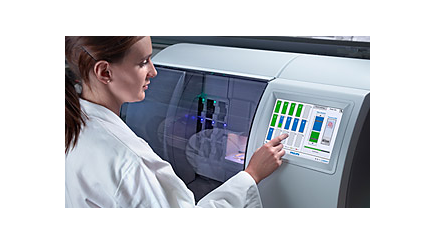
\includegraphics[width=0.8\textwidth]{PhilipsScanner.png}
\caption{Philips Scanner, each slide is scanned and exported to a tiff format.}
\label{PhilipsScanner}
\end{figure}
\begin{figure}[!ht]
\centering
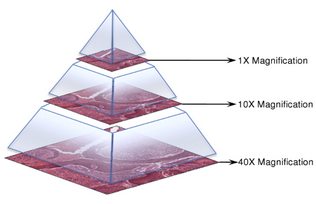
\includegraphics[width=0.8\textwidth]{pyramid.png}
\caption{Pyramid data Structure}
\textit{Between 8 and 10 different resolutions}
\label{Pyramid}
\end{figure}
Uncompressed one image can reach up to 65 GB, the WSI on the highest resolution had size 96256 x 218624 pixels and the lowest resolution had 188 x 427 pixels.
\subsubsection*{Machine learning core}

\subsubsection*{Post-processing}



\section{May 2016 and future work}



%\begin{figure}[!ht]
%\centering
%\includegraphics[width=\textwidth]{}
%\caption{}
%\label{}
%\end{figure}


\newpage

\begin{thebibliography}{9}

\bibitem{OriginalPaper} Thomas Bühler and Matthias Hein from Saarland University, Germany, \textit{Spectral Clustering based on the graph $p$-Laplacian}. ICML 2009.

\end{thebibliography}



\end{document}
